\section{ESPERIMENTI}
\justifying
In questa sezione sono riportati gli esperimenti eseguiti e le evidenze riscontrate. Ogni subsection relativa ad uno specifico esperimento riporta anche la descrizione delle pagine e delle policy definite \textbf{(cambia)}. Con il termine \textbf{importare} si fa riferimento all'incorporamento di una pagina web attraverso il tag HTML $<iframe>$ in una pagina definita \textit{parent page}. In Fig\ref{fig:ImgAttack} possiamo vedere una panoramica grafica degli esperimenti descritti di seguito. 

\begin{figure*}[t!]
    \centering
    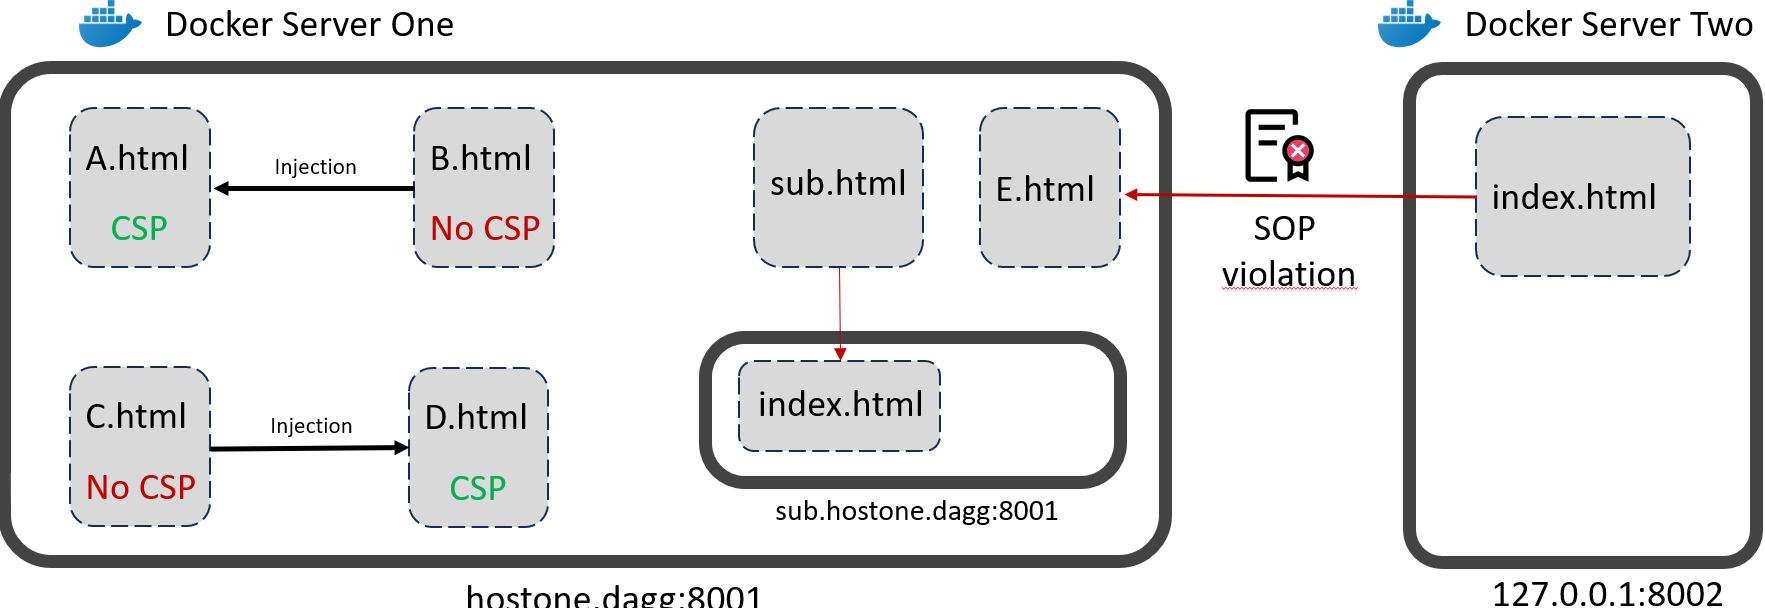
\includegraphics[width=0.9\textwidth]{Figuras/img_Attack.png}
    \caption{Panoramica degli esperimenti}
    \label{fig:ImgAttack}
\end{figure*} 

\subsection{Importazione da un dominio differente}
\label{par:dominiodifferente}
Lo scopo di questa casistica è quello di mostrare come effettivamente importare una pagina da un dominio differente sia un'azione che venga bloccata dalla policy SOP. Nel Server Two è stata creata una web page \textit{index.html} che presenta del testo ed esegue uno script-inline\footnote{Uno script inline è un codice JavaScript inserito direttamente all'interno di un TAG HTML, come il tag <script>. Viene eseguito dal browser non appena incontra il tag <script> durante il parsing della pagina web.} che tenta di visualizzare un messaggio di alert ("Codice JS iniettato") nella finestra parent (finestra importante) come si può vedere dal Listing \ref{importedJS}. 
\begin{lstlisting}[
    style=HTML,
    caption={Codice JS da eseguire su pagina parent},
    label=importedJS
]
                    ...
<script>
    window.parent.alert("Codice JS iniettato");
</script>
                    ...
\end{lstlisting}

La pagina E.html, presente nel Server One, si occuperà di effettuare la richiesta di importare tale pagina dal Server Two. Per farlo si utilzza il tag \textit{iframe} come in Listing\ref{}
\begin{lstlisting}[
    style=HTML,
    caption={Codice JS da eseguire su pagina parent},
    label=importedJS
]
                    ...
<iframe src="http://127.0.0.1:8002" 
        width="1000px" 
        height="240px">
</iframe>
                    ...
\end{lstlisting}
Tuttavia, questo codice non viene eseguito come previsto a causa di restrizioni delle restrizioni di sicurezza relative la Same Origin Policy. 
\begin{figure}[h!]
    \centering
    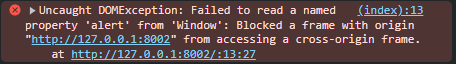
\includegraphics[width=0.4\textwidth]{Figuras/errori/E.html.error.png}
    \caption{Alert bloccato da SOP}
    \label{fig:ImgError1}
\end{figure} 
Nella console del browser possiamo vedere il messaggio di errore relativo, descritto dalla Fig.\ref{fig:ImgError1}.
Possiamo quindi concludere che si i due server creati hanno effettivamente due domini differenti e che SOP entri in gioco quando si tenta di accedere a risorse provenienti da domini diversi rispetto il dominio da cui parte la richiesta.

\subsection{Parent page con CSP, iframe senza CSP}
\label{par:csp_nocsp}
Lo scopo di questo esperimento è quello di verificare che nonostante in una pagina parent sia definita una policy CSP è possibile sfruttare gli iframe per importare una pagina sprovvista di CSP, quindi vulnerabile, ma che essendo proveniente dalla stessa origine, quindi lecita per SOP, venga importata e consenta l'injection di codice sulla pagina principale protetta bypassando il controllo della CSP. A tale scopo nell'head della pagina \textit{A.html}, attraverso il tag meta viene specificata la policy CSP Listing \ref{CSPa_b}.
\begin{lstlisting}[
    style=HTML,
    caption={Page A CSP policy},
    label=CSPa_b
]
                    ...
<meta   http-equiv="Content-Security-Policy" 
        content="script-src 'self'">
                    ...
\end{lstlisting}
Attraverso la seguente policy, con l'attributo \textit{"script -src ’self ’"} si va a specificare come all'interno della pagina siano possibile eseguire solamente script provenienti dalla stesso dominio, tuttavia non è possibile andare ad eseguire script-inline in quanto questi richiederebbero la definizione dell'attributo 'unsafe-inline'. Importanto la pagina \textit{B.html} attraverso il codice Listing \ref{importbina} possiamo avere evidenza di come il codice java script (Listing\ref{inlineB}) presente all'interno dei tag inline $<script>$ riescano ad essere eseguiti all'interno della pagian parent A.html ed anche ad accedere agli elementi del DOM per andare in questo caso ad accedere ad una variabile 'secret' presente nel codice di A.html. 
\begin{lstlisting}[
    style=HTML,
    caption={Iframe della pagina B.html in A.html},
    label=importbina
]
                    ...
 <iframe src="B.html" ... "></iframe>
                    ...
\end{lstlisting}
\begin{lstlisting}[
    style=HTML,
    caption={Script inline di B.html per accedere a secret},
    label=inlineB
]
                    ...
<script>
    window.onload = function () {
        var parentWindow = window.parent;
        var secretValue = parentWindow.secret;
                    ...
\end{lstlisting}
Possiamo quindi notare come sia possibile sfruttare una pagina importata e non protetta da CSP per andare a fare l'injection di codice malevolo che verrà quindi propagato all'interno di una pagina protetta da CSP, in quanto questa policy non verrà propagata alla pagina importata e lo script malevolo non sarà a sua volta bloccato da SOP in quanto proveniente dalla stessa origine. 
\subsection{Parent page senza CSP, iframe con CSP}
\label{par:nocsp_csp}
In questa sezione si va a verificare come sia possibile accedere alla variabile secret di D.html andando a sfruttare l'import tramite iframe della pagina D.html, ma accedendoci maliziosamente questa volta dalla pagina parent C.html. Nello specifico abbiamo che la pagina parent C.html non è protetta da alcun CSP, mentre la pagina child D.html presenta il CSP definiti in Listing \ref{CSPa_b}. L'import della pagina D.html nella parent page C.html avviene attraverso l'iframe descritto nel Listing \ref{frameD}. 
\begin{lstlisting}[
    style=HTML,
    caption={Import di D.html in C.html},
    label=frameD
]
                    ...
<iframe id="d_frame_id" src="D.html"></iframe>
                    ...
\end{lstlisting}
In questo caso abbiamo che all'iframe è stato associato un id \textit{d\_frame\_id}, questo ci permetterà di far riferimento al frame e di manipolare le risporse all'interno dell'iframe tramite java script. In questo esempio per accedere alla variabile segreta in facciamo eseguire il codice JS descritto nel Listing \ref{CJSinj}. Questo codice attende che l'iframe sia effettivamente caricato nella parent page per poi andare tramite l'identificativo ad accedere alla variabile secret. Infine nelle righe 6 e 7 andiamo ad eseguire un alert all'interno della pagina importata. 
\begin{figure*}[t!]
\begin{lstlisting}[
    style=HTML,
    caption={Codice JS di C.html per accedere alle risorse della child page D.html},
    label=CJSinj
]
                                                ...
<script>
    window.onload = function() {
        child_frame = document.getElementById("d_frame_id");
        secret_D = child_frame.contentWindow.secret;
        child_frame.contentWindow.postMessage(
            alert("Codice JS iniettato nell'iframe" + secret_D), "*"); 
        };
</script> 
                                                ...
\end{lstlisting}
\end{figure*}
Possiamo quindi notare come anche in questo caso si riesca a raggirare la policy CSP e a fare eseguire dello script inline nonostante i controlli nella pagina importata vadano a bloccarne l'esecuzione. Questo può essere sfruttato andando ad iniettare all'interno della pagina parent, priva di controlli e vulnerabile, del codice malevolo, ad esempio nella forma di scripting-inline che verrà poi propagato ed iniettato nella pagina importata rendendola a sua volta una pagina vulnerabile. Se si volesse fare l'injection del codice malevolo solamente nella pagina importata, questo verrebbe bloccato dalla CSP. 
\subsubsection{Check script inline non eseguibili}
Nel Framework viene mostrato come gli script inline delle pagine che implementano CSP siano effettivamente disattivati, per farlo lo si mostra tramite il pulsante di ritorno ad Home, definito attraverso degli script inline. Anche dopo aver eseguito l'attacco, la logica del bottone non è operativa, mentre andando ad inserire la direttiva \textbf{'unsafe-inline'} all'interno dell'header delle pagine il bottone diventi operativo. 

\subsection{Importare da un sottodominio}
\label{par:subdomainex}
Come descritto in questa sezione si descrive il caso in cui una pagina index.html appartenente al sottodominio \textit{sub.hostone.dagg:8001} viene importata all'interno di una pagina sub.html eseguita nel Server One quindi al dominio \textit{hostone.dagg:8001}. Come descritto nel capitolo \ref{Origin} i due domini seppur condividendo lo stesso dominio di secondo livello sono in realtà considerati da SOP come due origini differenti. Lo scopo di questo esperimento era appunto quello di voler mostrare come l'import di una pagina di un sottodominio venga appunto bloccata da SOP e successivamente andare a valutare come l'utilizzo della direttiva \textit{document.domain} nell'ambiente obsoleto permetteva appunto di poter raggirare tale restrizione mentre come oggi non sia possibile in ambiente odierno in quanto nel corso degli anni la direttiva è stata deprecata\cite{5}. Nell'andare ad eseguire l'import in tutti i casi il JS viene iniettato dalla pagina del sottodomini alla pagina principale. Quindi il SOP non entra in gioco per bloccare la violazione. Procedendo all'analisi degli header nella console del browser, in immagine \ref{fig:Headers}, possiamo notare dal campo 'Referer' come la richiesta avviata dal dominio \textit{hostone.dagg:8001} sia diretta verso il dominio \textit{sub.hostone.dagg:8001} come specificato dal campo 'Host'. Dunque effettivamente i due domini sono due domini differenti. 
\begin{figure}[h!]
    \centering
    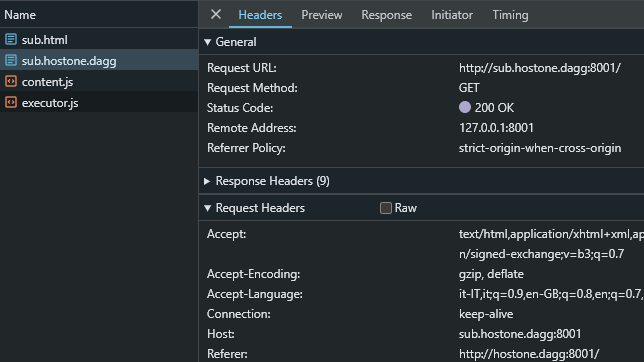
\includegraphics[width=0.4\textwidth]{Figuras/errori/network-sub-domains.png}
    \caption{Attributi Request Headers di hostone.dagg}
    \label{fig:Headers}
\end{figure} 
Successivamente con l'obiettivo di definire la possibilità del server di poter accettare o meno richieste da domini differenti si è proceduto andando a definire la CSP non più a livello di singola pagina ma a livello di header-server, nello specifico, all'interno del file di configurazione Apache \textit{000-default.conf} sono state aggiunte le due istruzioni: 
\begin{center}
    \begin{small}
    Header set Access-Control-Allow-Origin "hostone.dagg:8001/"\\
    Header always set Content-Security-Policy "script-src 'self' 'unsafe-inline'"
    \end{small}
\end{center}
Rimuovendo le definizioni delle CSP precedentemente descritte nei paragrafi \ref{par:csp_nocsp} e \ref{par:nocsp_csp} e riavviando il server abbiamo che i controlli continuano ad essere eseguiti dunque la policy CSP viene applicata a tutte le pagine web del server, ma il problema relativo non è stato risolto nonostante sia stata definita fortemente l'origine tramite il primo comando.

\subsection{Comparazione sui diversi ambienti e browser}
Per quanto riguarda l'esecuzione degli esperimenti sui due ambienti descritti nel paragrafo \ref{AmbienteObsoleto} non si sono notate differenze. Successivamente si sono replicati gli esperimenti sui diversi browser elencati in tabella \ref{tab:browser}. 
\begin{table}[h!]
\centering
\caption{Browser e versioni}
\label{tab:browser}
   \begin{tabular}{|cc|}
   \rowcolor{gray!30}
   \hline
    \textbf{Browser} & \textbf{Versione} \\
    \hline
    Chrome & 122.0.6261.112 \\
    Edge & 122.0.2365.80 \\
    Opera & 122.0.6261.95 \\
    Firefox & 123.0.1 \\
    \hline
\end{tabular}
\end{table}
Su tutti i browser si sono osservati gli stessi comportamenti e risultati descritti nei capitoli \ref{par:dominiodifferente}, \ref{par:csp_nocsp}, \ref{par:nocsp_csp}, \ref{par:subdomainex}. 